\documentclass[si.tex]{subfiles}
\begin{document}

%\textcolor{red}{TODO probably throughout we want to say 'Bias' instead of 'Total'}


We provide extensive simulations for a variety of models on circular and interval spaces, expanding on Figures 4 and 5 in the main text.

\subsection{Operationalization of Attraction and Repulsion}\label{sec:att-rep}

Throughout the SI Appendix, we visualize not only the overall fitted bias, but also its decomposition into Attraction and Repulsion components.
As shown in \cite{hahn2024unifying}, the bias for the $L_p$ estimator has the form
\begin{equation}\label{eq:ana-bias-att-rep}
    \text{Bias}(\theta) = \underbrace{\frac{1}{\FI(\theta)} (\log \Prior(\theta))'}_{\text{Prior Attraction}} + \underbrace{\frac{p+2}{4} \left(\frac{1}{\FI(\theta)}\right)'}_{\text{Likelihood Repulsion}} + \mathcal{O}(\sigma^4)
\end{equation}
when $p > 0$, and
\begin{equation}\label{eq:ana-bias-att-rep-0}
    \text{Bias}(\theta) = \underbrace{\frac{1}{\FI(\theta)} (\log \Prior(\theta))'}_{\text{Prior Attraction}} + \underbrace{\frac{1}{4} \left(\frac{1}{\FI(\theta)}\right)'}_{\text{Likelihood Repulsion}} + \mathcal{O}(\sigma^4)
\end{equation}
in the case $p=0$.

The first component expresses classical attraction  to the prior, traditionally considered a hallmark of Bayesian models.
The second component expresses repulsion away from regions allocated high encoding resources, towards stimuli that are less well encoded; it appears because such inhomogeneities in encoding precision make the posterior asymmetric \citep{Wei2012,Wei2015ABO,Wei2017LawfulRB,PratCarrabin2021BiasAV,hahn2024unifying}.

This decomposition of the bias clarifies how prior, encoding, and loss function jointly determine the bias.
Our theoretical and simulation results indicate that the decomposition can be reliably recovered from behavioral data.
To illustrate this, thoughout the SI Appendix, we visualize not only the fitted overall bias, but also the attraction and repulsion components.
As the decomposition is exact only in the low-noise limit (indicated by the $\mathcal{O}(\sigma^4)$ residual term), we require an operationalization of the decomposition that is adapted to larger noise levels.
To achieve this, we follow \cite{hahn2024unifying} in operationalizing the attraction component as the decoding bias ($\mathbb{E}[\mathbb{\widehat{\theta}}|m] - F^{-1}(m)$) for the MAP estimator ($p=0$), which has the analytical form
\begin{equation}
    \frac{1}{\FI(\theta)} (\log \Prior(\theta))' + \mathcal{O}(\sigma^4)
\end{equation}
matching the Prior Attraction up to a higher-order residual.
Also following \cite{hahn2024unifying}, we operationalize the repulsion component as the difference between the overall prior and this component.
By definition, and in accordance with the analytical decomposition (\ref{eq:ana-bias-att-rep}--\ref{eq:ana-bias-att-rep-0}), the attractive component is independent of the loss function, whereas the repulsive component depends on it.
In the special case where encoding is exactly uniform, we instead plot the full bias as attraction, with a zero repulsive component (following \cite{hahn2024unifying}; Figure~\ref{fig:recover-model-circ-periodic-uniform}).
As in \cite{hahn2024unifying}, separate visualization of these components via such an operationalization serves an illustrative purpose, but we caution that there may be other possible operationalizations of the components in the finite-noise regime.

\paragraph*{Difference between Analytical and Plotted Components}
We note that, while this operationalization provides a general idea of the decomposition, it reflects higher-order information of the residual $\mathcal{O}(\sigma^4)$ and thus sometimes shows behavior not expected of the two components in the analytical decomposition (\ref{eq:ana-bias-att-rep}--\ref{eq:ana-bias-att-rep-0}). Specifically, the plotted repulsive component may somewhat depend on the prior because, as noise becomes larger, the prior can impact the higher-order residual $\mathcal{O}(\sigma^4)$. As a consequence, even if the encoding is near-uniform and the repulsion is zero in the small-noise limit, the plotted repulsive component at large noise need not be zero.

\paragraph*{Behavior in Interval Stimulus Spaces}
In interval stimulus spaces, close to the boundary, the bias receives an additional term, indicating a regression effect into the interior of the interval (Theorem 3 in \cite{hahn2024unifying}).
The operationalization of attraction and repulsion described above naturally partitions this regression effect into components grouped with attraction and repulsion, respectively. Thus, rather than separately plotting the regression effect as a third component, we plot attraction and repulsion components that both include portions of the boundary effect, as determined by the operationalization.


%\textcolor{red}{TODO make sure it's done like this in all plots}


\subsection{Models on Circular Spaces (Supplement to Figure 5)}
For circular spaces, we investigate the following combinations:
\begin{enumerate}
\item Periodic encoding and uniform prior (Figures~\ref{fig:recover-model-circ-uniform-periodic} and \ref{fig:recover-loss-circ-uniform-periodic})
\item Periodic encoding and periodic (shifted) prior (Figures~\ref{fig:recover-model-circ-shifted-periodic} and  \ref{fig:recover-loss-circ-shifted-periodic})
\item Periodic encoding and periodic prior (Figures~\ref{fig:recover-model-circ-periodic-periodic} and  \ref{fig:recover-loss-circ-periodic-periodic})
\item Uniform encoding and periodic prior (Figures~\ref{fig:recover-model-circ-periodic-uniform} and  \ref{fig:recover-loss-circ-periodic-uniform})
\end{enumerate}
Across settings, we find that the encoding and prior are closely fitted when given the correct loss function, and that the loss function is closely identified when the number of noise levels and trials is sufficiently large.
Further, in Figure~\ref{fig:circular-gauge}, we provide an explicit example of models with different loss functions and priors that have the same response distribution in the limit of zero noise.



\subfile{si-fits-by-p-circular}
\subfile{si-figure5-circular}

\begin{figure}


\begin{center}

$p=0$

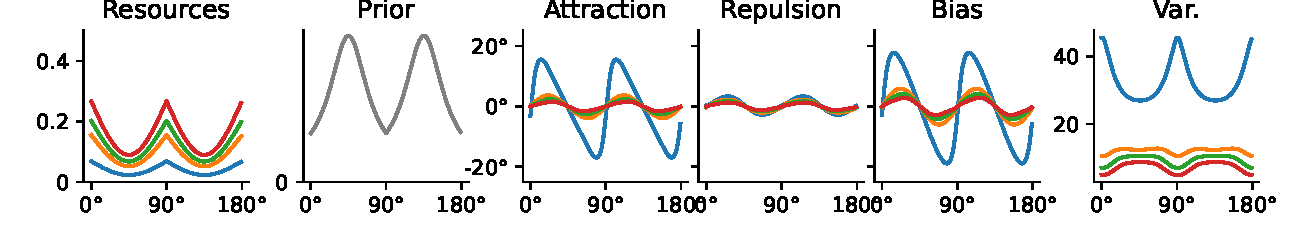
\includegraphics[width=0.5\textwidth]{figures/CounterfactualModel_VIZ_ByNoiseMagnGauge.py_2345_UNIFORM_STEEPPERIODIC_0_0_10.0_180.pdf}


$p=1$

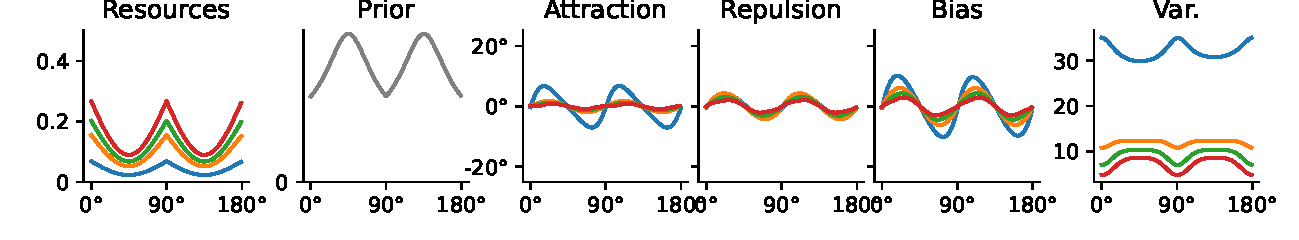
\includegraphics[width=0.5\textwidth]{figures/CounterfactualModel_VIZ_ByNoiseMagnGauge.py_2345_UNIFORM_STEEPPERIODIC_1_0_10.0_180.pdf}


$p=2$

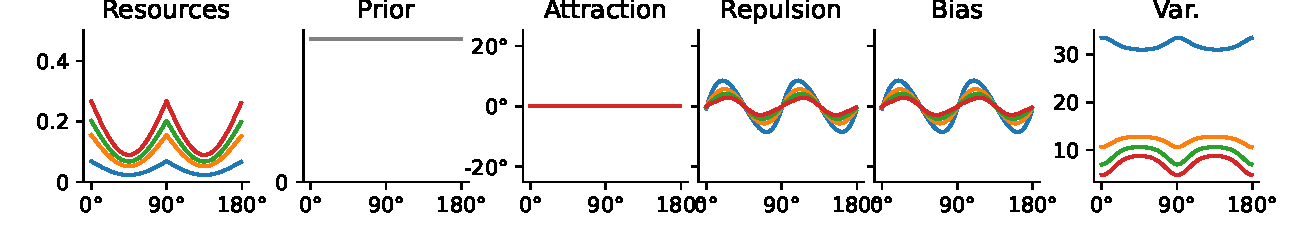
\includegraphics[width=0.5\textwidth]{figures/CounterfactualModel_VIZ_ByNoiseMagnGauge.py_2345_UNIFORM_STEEPPERIODIC_2_0_10.0_180.pdf}

$p=4$

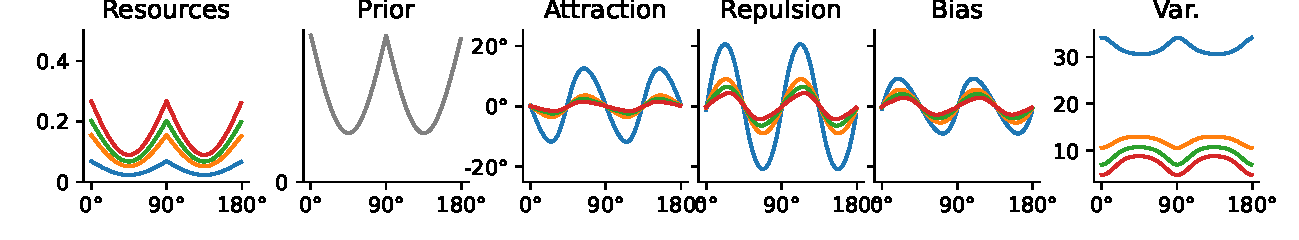
\includegraphics[width=0.5\textwidth]{figures/CounterfactualModel_VIZ_ByNoiseMagnGauge.py_2345_UNIFORM_STEEPPERIODIC_4_0_10.0_180.pdf}

$p=6$


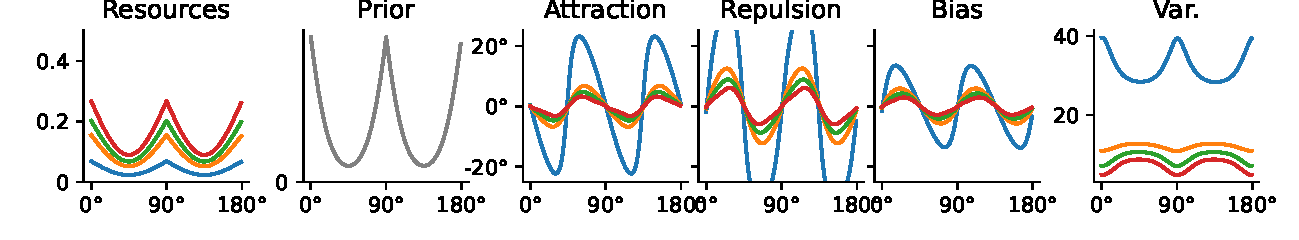
\includegraphics[width=0.5\textwidth]{figures/CounterfactualModel_VIZ_ByNoiseMagnGauge.py_2345_UNIFORM_STEEPPERIODIC_6_0_10.0_180.pdf}

$p=8$


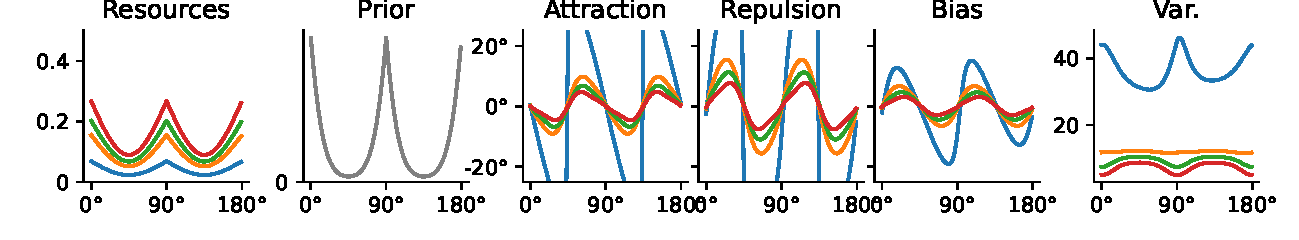
\includegraphics[width=0.5\textwidth]{figures/CounterfactualModel_VIZ_ByNoiseMagnGauge.py_2345_UNIFORM_STEEPPERIODIC_8_0_10.0_180.pdf}

\end{center}

\begin{comment}
for i in {0,1,2,4,6,8} ; do python3 CounterfactualModel_VIZ_ByNoiseMagnGauge.py $i 0 10.0 180 UNIFORM STEEPPERIODIC 2345 ; done
\end{comment}
\caption{Models that have the same response distribution in the limit of zero noise (same encoding; prior transformed by Eq. 3), but different behavior for nonzero noise.
For such models, the loss function may be poorly identified at one level of sensory noise, but well identified when more levels of sensory noise are available (see Figure~\ref{fig:recover-loss-circ-uniform-periodic}).
Theorems 3--4 show that this situation is typical for most combinations of prior and encoding.
}\label{fig:circular-gauge}
\end{figure}



\subfile{si-effect-noise-levels}


\subsection{Models on Interval Spaces}\label{sec:further-interval}
For interval spaces, we investigate the following combinations:
\begin{enumerate}
\item Unimodal encoding and uniform prior (Figures \ref{fig:fit-uniform-unimodal} and \ref{fig:uniform-unimodal})
\item Unimodal encoding and unimodal prior (Figures \ref{fig:fit-unimodal-unimodal} and \ref{fig:unimodal-unimodal})
\item Bimodal encoding and uniform prior (Figures \ref{fig:fit-uniform-bimodal} and \ref{fig:uniform-bimodal})
\item Uniform encoding and unimodal prior (Figures \ref{fig:fit-unimodal-uniform} and \ref{fig:unimodal-uniform})
\end{enumerate}
Across settings, we find that the encoding and prior are closely fitted when given the correct loss function, and that the loss function is closely identified when the number of noise levels and trials is sufficiently large.

\subfile{si-fits-by-p-interval}
\subfile{si-figure5-interval}


\subsection{Randomly Generated Models (Supplement to Figure 4)}
We provide additional extensive simulations complementing Main Text Figure 4 in  Figures \ref{fig:fourier-0}--\ref{fig:fourier-8}, with three randomly generated model at each loss function exponent.
Across the board, encodings, priors, and loss functions are recovered.



\paragraph*{Random Model Generation}
For each of the random models, we initialized Python's \texttt{random} generator with a three-digit seed determined as follows: The first digit is 1 for the prior and 2 for the encoding. The second digit is the loss function. The third digit is 1, 2, 3, giving us a total of three random models per loss function exponent.

We then sampled the encoding and prior each by setting
\begin{equation}
\sum_{i=0}^4 \left( X_i \sin(i \theta_i) + Y_i \cos(i \theta_i) \right)
\end{equation}
where $X_i, Y_i \sim Uniform([-0.5, 0.5])$ drawn using the \texttt{random()} function, and applying the softmax function to the resulting vector to obtain an element of $\mathcal{F}(\mathcal{X})$.



\subfile{si-figure4-circular}


\end{document}
